\chapter{Random Forests, Ferns, Meta-Algoritmi}

\section{Meta algoritmi nel machine learning}
Un meta-algoritmo, nel contesto del machine learning, rappresenta un modo di combinare più modelli, detti \textit{weak learner} .
Tra questi, studiamo

\paragraph{Tree hierarchy} Definita come una gerarchia di domande (\textit{weak learner}). Ogni nodo è un modello. La struttura ad albero permette di soezzare lo spazio delle feature in varie regioni. I decision tree classifici rappresentano un caso particolare di questo meta-algoritmo. È una struttura facile da interpretare (\textit{if-then-else}). Un albero decisionale è una particolare istanza di questo.

\paragraph{Bagging (Bootstrap Aggregating)} Migliora i modelli di classificazione, in termini di stabilità e precisione. Riduce la varianza e permette di evitare l'overfitting.
Dato un traning set $I$ di dimensione $n$, il bagging genera $m$ nuovi training set $I_i$, ognuno di essi di dimensione $n' < n$, campionando esempi da $I$\footnote{Potrebbe ricordare la $k$-fold validation. Tuttavia, se il bagging  è un metodo per ridurre l'overfitting, la cross validation viene utilizzata per stimare l'accuratezza del modello fuori dal campione di training.}. Ciascuno dei sotto-training set allena un modello differente. L'output complessivo è una media o una votazione.

\paragraph{Boosting} Gli algoritmi di boosting consistono nell'allenare iterativamente dei classificatori deboli secondo una distribuzione. Questi vengono poi aggiungi al classificatore complessivo in maniera pesata (\textit{"quanto conta questo classificatore nella valutazione complessiva?"}). Il peso è solitamente proporzionale all'accuracy del singolo modello.


Trattiamo questi meta-algoritmi, in quanto permettono di ottenere dei modelli strutturalmente semplici, ma sempre più precisi e meno proni a overfitting.

\section{Decision stump - Ceppo di decisione}

È un albero decisionale a singolo nodo. Può essere univariato o multivariato. Data la loro semplicità, sono dei classificatori lineari. Saranno i nostri \textit{weak learners}. 

\begin{figure}[tbph]
	\centering
	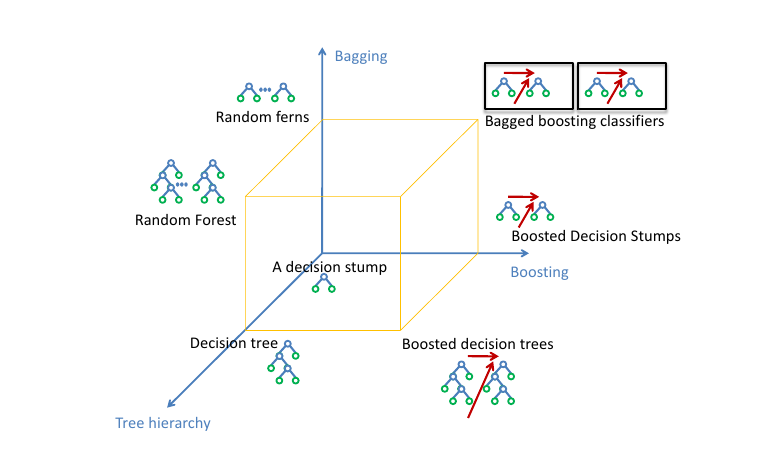
\includegraphics[width=\linewidth]{images/meta-algorithm-trees}
	\caption{Meta-Algoritmi applicati sui decision stump.}
\end{figure}


\section{Decision Trees}
Applichiamo la \textbf{tree hierarchy} sui nostri decision stump, ottenendo una gerarchia di decisioni. Tramite una serie di domande di tipo "yes/no", o varie sogliature, diventa possibile classificare categorie sempre più specifiche. Ogni coppia di risultati di un nodo di un decision tree, è detta \textit{split}. La profondità (direttamente proporzionale al numero di split), definisce la complessità del modello. Alberi decisionali troppo profondi rischiado di cadere in overfitting.

\section{Random Ferns}
Bagging applicato sugli stump ci fa ottenere i random ferns. Questi hanno riscontrato molte applicazioni in task di object detection, tramite previa suddivisione delle immagini in patches. La semplicità dei singoli fern offre possibilità di parallelizzazione piuttosto banale. Riprendono le intuizioni dietro i classificatori bayesiani\footnote{Un classificatore bayesiano è un classificatore basato sull'applicazione del teorema di Bayes. Il classificatore bayesiano richiede la conoscenza delle probabilità a priori e condizionali relative al problema, quantità che in generale non sono note ma sono tipicamente stimabili.}.

\section{Random Tree}
Un random tree è un decision tree costruito con dei parametri scelti da un insieme di proposte casuali. Per ogni nodo, un set di linee viene valutato, e il rispettivo parametro viene fissato nel modello. L'obiettivo a ogni passo è massimizzare l'informazione ottenuta a ogni passo. 

\subsection{Randomized learning}
Si utilizza un algoritmo ricorsivo. 


$$
\text{Left split: } I_1 = \{i \in I_n | f(v_i) < t\} \qquad \text{Right split: } I_r =  I_n \setminus I_1
$$

con $t$ soglia, treshold scelta dal range del minimo e del massimo di $f(v_i)$. L'obiettivo è ottenere il massimo guadagno di informazione, ossia

$$
\Delta E = -\frac{|I_l|}{|I_n|}E(I_1) -\frac{|I_r|}{|I_n|}E(I_r)
$$

\section{Random forest}
Le random forest nascono dall'unione delle intuizioni relative al bagging e alla tree hierarchy. Si basano sulla combinazione di output di più decision trees (spesso random trees) per ottenere un unico risultato. La loro facilità d'uso e la  flessibilità ne hanno favorito l'adozione, e possono essere usate sia su task di classificazione che di regressione.  Offrono un ottimo grado di \textbf{precisione}, \textbf{cadono meno facilmente in overfitting} e sono assolutamente \textbf{multi-core friendly}.

\begin{figure}[tbph]
	\centering
	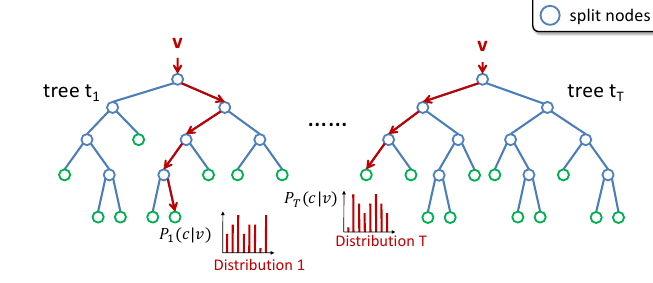
\includegraphics[width=1\linewidth]{images/random-forest}
\end{figure}

La classificazione è ottenuta considerando la distribuzione media computata dalle foglie.

$$
\frac{1}{T} \sum_{t=1}^{T}P_t(c|v)
$$





